\section{Intuição}

Um objeto a uma temperatura $T>T_{amb}$ irá dissipar energia sob a forma de calor para a vizinhança espontaneamente. A energia interna do objeto diminuirá, enquanto a energia interna do ambiente aumentará, até se atingir o equilíbrio. O processo inverso não ocorre espontaneamente.
Embora em termodinâmica estatística, numa análise microscópica, pode-se considerar que atomicamente a energia pode ser transmitida entre os átomos em ambas as direções, mas sendo o resultado final o aumento da energia do átomos do ambiente.

Um balanço de energia não nos diz a direção de um processo espontâneo, assim como a rapidez com que se atinge o equilíbrio. Para isso, é necessário a segunda lei da termodinâmica.

É de notar que sempre que existe um desiquilíbrio entre dois sistemas, existe uma oportunidade de se desenvolver trabalho, que seria irrevogavelmente perdido se se deixasse que o equilíbrio fosse atingido de forma descontrolada. Por exemplo, existindo uma diferença de pressão poder-se-á produzir trabalho com uma turbina, ou numa barragem hidroelétrica, a diferença de altura entre os reservatórios de água também pode e é aproveitado para a produção de energia elétrica.


A segunda lei da termodinâmica permite calcular o trabalho máximo teórico que se pode obter num dado processo.


\section{Formulação de Clausius - 1850}

\begin{theorem}[Clausius]
    É impossível que um dado sistema opere de tal foram que o único resultado seja a transferência de energia sobre calor de um reservatório fria para um quente.
\end{theorem}


De forma equivalente, ``Quando dois reservatórios se aproximam, existe um fluxo de espontâneo de energia sob a forma de calor do que tem maior temperatura para o de menor temperatura.''


\section{Formulação de Kelvin-Planck - 1855}

\begin{theorem}[Kelvin-Planck] \label{thm:kelvin-planck}
    É impossível que um dado sistema opere num ciclo termodinâmico de tal forma que realize trabalho útil na sua vizinhança, enquanto recebe energia de um único reservatório térmico.
\end{theorem}

É claro que isto não impede a possibilidade de um sistema realizar trabalho, devido a uma transferência de calor de um único reservatório. Apenas rejeita que tal seja possível durante um ciclo completo.

Este enunciado já não é tão evidente. No entanto, pode-se demonstrar que as formulações de Clausius e de Kelvin-Planck são \textbf{equivalentes}. Para isso, mostra-se que a violação de uma implica a violação da outra:

\begin{itemize}
    \item $\sim \textbf{Clausius} \implies \sim \textbf{Kelvin-Planck}$: Considerando que num sistema é possível ocorrer uma transferência espontânea de calor de um reservatório frio para um quente ($\sim \textbf{Clausius}$) (ver Figura \ref{fig:eq-clausius-kelvin}), poderemos adicionar um outro sistema entre os mesmos dois reservatórios que opera num ciclo, que recebe $Q_H$ do reservatório quente e cede $Q_C$ para o frio, realizando trabalho $W_u$ para a vizinhança. O balanço energético deste sistema dá-nos que $W_u = Q_H - Q_C$. No entanto, se fizermos um balanço energético para um sistema cuja fronteira inclui os dois sistemas considerados e que coincide com a fronteira com o reservatório quente e inclui o reservatório frio, sabemos que o sistema recebe $Q_H$ e cede $Q_C$ para o reservatório quente (resultante do fluxo espontâneo de calor que considerámos possível), i.e. recebe $Q_H - Q_C$. Desta forma, no total, o sistema recebe $Q_H - Q_C$ de um único reservatório e realiza trabalho na vizinhança igual a $Q_H - Q_C$. Ora, isto viola a formulação de Kelvin-Planck. \\ 
    
    \begin{figure}[H]
        \centering
        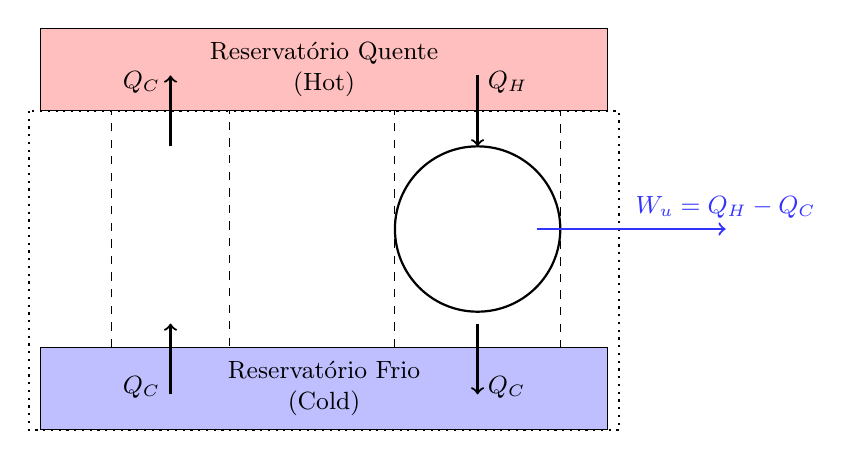
\begin{tikzpicture}[scale=1.5, every node/.style={font=\small}]
            % Colors
            \filldraw[fill=red!25] (-2.4,1) rectangle (2.4,1.7);
            \filldraw[fill=blue!25] (-2.4,-1.7) rectangle (2.4,-1);

            \node[text width=3.5cm, align=center] at (0,1.35) {Reservatório Quente\\(Hot)};
            \node[text width=3cm, align=center] at (0,-1.35) {Reservatório Frio\\(Cold)};


            % Sistema em ciclo termodinâmico (círculo)
            \draw[thick] (1.3,0) circle (0.7);

            % Linhas pontilhadas definindo o sistema combinado
            \draw[dotted, thick] (-2.5,1) rectangle (2.5,-1.7);

            % Caixas verticais (fronteiras internas)
            \draw[dashed] (-1.8,-1) rectangle (-0.8,1);
            \draw[dashed] (0.6,-1) rectangle (2,1);

            % Setas de calor
            \draw[->, thick, black] (-1.3,0.7) -- (-1.3,1.3) node[pos=0.9, left] {$Q_C$};
            \draw[->, thick, black] (-1.3,-1.4) -- (-1.3,-0.8) node[pos=0.1, left] {$Q_C$};

            \draw[->, thick, black] (1.3,1.3) -- (1.3,0.7) node[pos=0.1, right] {$Q_H$};
            \draw[->, thick, black] (1.3,-0.8) -- (1.3,-1.4) node[pos=0.9, right] {$Q_C$};

            % Seta de trabalho
            \draw[->, thick, blue!80] (1.8,0) -- (3.4,0) node[pos=1, above] {$W_{u} = Q_H - Q_C$};

        \end{tikzpicture}
        \caption{Ilustração da $\sim \textbf{Clausius} \implies \sim \textbf{Kelvin-Planck}$}
        \label{fig:eq-clausius-kelvin}
    \end{figure}
    
    \item $\sim \textbf{Kelvin-Planck} \implies \sim \textbf{Clausius}$: Considerando um sistema que opera num ciclo recebendo $Q_H$ de um único reservatório quente e realiza trabalho igual a $W_u = Q_H$ ($\sim \textbf{Kelvin-Planck}$), e que esse trabalho é usado para operar um ciclo frigorífico que remove $Q_C$ de um reservatório frio e transfere $Q_H'$ para o mesmo reservatório quente. O balanço energético deste ciclo dá-nos que $W_u = Q_H' - Q_C$, pelo que $Q_H = Q_H' - Q_C \Leftrightarrow Q_H' = Q_H + Q_C$. Novamente, fazendo o balanço energético global para os dois sistemas, obtemos que na interação com o reservatório frio recebe $Q_C$. Na interação com o reservatório quente, no ciclo que viola Kelvin-Planck recebe $Q_H$ e cede $Q_H' = Q_H + Q_C$, no ciclo frigorífico, i.e. cede $Q_H' - Q_H = Q_C$ ao reservatório quente. Na verdade, trata-se de único fluxo de calor igual a $Q_C$ de um reservatório frio para um reservatório quente. Ora, isto viola a formulação de Clausius.

    \begin{figure}[H]
        \centering
        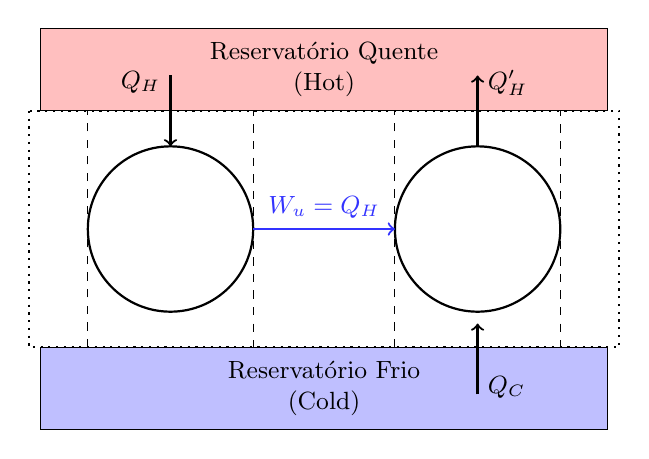
\begin{tikzpicture}[scale=1.5, every node/.style={font=\small}]
            % Colors
            \filldraw[fill=red!25] (-2.4,1) rectangle (2.4,1.7);
            \filldraw[fill=blue!25] (-2.4,-1.7) rectangle (2.4,-1);

            \node[text width=3.5cm, align=center] at (0,1.35) {Reservatório Quente\\(Hot)};
            \node[text width=3cm, align=center] at (0,-1.35) {Reservatório Frio\\(Cold)};


            % Sistema em ciclo termodinâmico (círculo)
            \draw[thick] (1.3,0) circle (0.7);
            \draw[thick] (-1.3,0) circle (0.7);

            % Linhas pontilhadas definindo o sistema combinado
            \draw[dotted, thick] (-2.5,1) rectangle (2.5,-1);

            % Caixas verticais (fronteiras internas)
            \draw[dashed] (-2,-1) rectangle (-0.6,1);
            \draw[dashed] (0.6,-1) rectangle (2,1);

            % Setas de calor
            \draw[->, thick, black] (-1.3,1.3) -- (-1.3,0.7) node[pos=0.1, left] {$Q_H$};

            \draw[->, thick, black] (1.3,0.7) -- (1.3,1.3) node[pos=0.9, right] {$Q_H'$};
            \draw[->, thick, black] (1.3,-1.4) -- (1.3,-0.8) node[pos=0.1, right] {$Q_C$};

            % Seta de trabalho
            \draw[->, thick, blue!80] (-0.6,0) -- (0.6,0) node[midway, above] {$W_{u} = Q_H$};

        \end{tikzpicture}
        \caption{Ilustração da $\sim \textbf{Kelvin-Planck} \implies \sim \textbf{Clausius}$}
        \label{fig:eq-kelvin-clausius}
    \end{figure}

\end{itemize}

Conclui-se, assim, que $\textbf{Clausius} \Longleftrightarrow \textbf{Kelvin-Planck}$, Q.E.D.

\section{Entropia}

A entropia é uma propriedade extensiva, como a massa e energia. Tal como as anteriores, a entropia pode ser transferia pela fronteira de um sistema. Para sistemas fechados, a transferência de entropia acompanha a transferência de calor. Em volumes de controlo, pode adicionalmente ocorrer pelos fluxos de matéria que entrem e saem.

\begin{theorem}[Entropia]
    É impossível que um dado sistema opere de tal forma que a entropia seja destruída.
\end{theorem}

Um processo é \textbf{irreversível} se o sistema e a vizinhança não podem ser restaurados ao seu estado inicial após esse processo. Um processo é \textbf{reversível} caso contrário. Num processo irreversível, é possível que o sistema retorne ao estado inicial, mas não é possível que a vizinhança também retorne.

Pode-se concluir que qualquer processo que envolva uma transferência de calor de um corpo quente para um frio é irreversível. Caso contrário, seria possível devolver a energia por calor do corpo frio para o quente sem quaisquer outros efeitos nos dois corpos. Ora, isto é impossível, pois viola a Formulação de Clausius. Outros exemplos de irreversibilidades são: a expansão de um gás para um local de baixa pressão, reação química espontânea, atrito, corrente elétrica passando por uma resistência, magnetização e polarização com histerese, e deformação inelástica.

Isto sugere que todos os processos são irreversíveis. A reversibilidade só é possível num processo infinitamente lento, ou de \textbf{quase-equilíbrio} (ou quase estático), onde o sistema passaria por sucessivos estados de equilíbrio.

Por exemplo, um êmbolo que comprime um gás adiabaticamente num cilindro sem atrito, numa compressão lenta, um pequeno aumento da pressão exterior, leva o êmbolo a comprimir ligeiramente o gás. Em cada estado intermediário, as propriedades intensivas $T$, $p$, $v$, etc, mantém-se uniformes, i.e. o gás passa por uma série de estados de equilíbrio. Por consequência, quando o êmbolo voltasse à posição inicial, o gás voltaria ao estado inicial. Assim, o trabalho feito na compressão do gás seria igual ao trabalho que o gás realizaria de volta na sua expansão livre. 

Matematicamente, $\delta W = - F dx = -\frac{F}{A} A dx = -p_{int} dV$. Sabemos que $\sum F = m \frac{dv}{dt} \Longleftrightarrow \frac{F_{int} - F_{ext}}{A} = \frac{m}{A}\frac{dv}{dt} \implies p_{int} - p_{ext} = \frac{m}{A} \frac{dv}{dt}$. Assim, num processo lento, $dt \to \infty \implies p_{int} \approx p_{ext}$

Um pêndulo ideal, sem atrito no pivô, no vácuo, é um movimento reversível, dado que a cada período o mesmo estado, a mesma altura, é atingida pelo pêndulo e na vizinhança.

Num processo \textbf{internamente reversível} não há irreversibilidades dentro do sistema, podendo, no entanto, haver na vizinhança. Deste modo, qualquer processo sob um reservatório térmico é internamente reversível.

\section{Forma analítica de Kelvin-Planck}

Um ciclo é reversível se todos os processos do ciclo forem reversíveis.

A forma analítica da Formulação de Kelvin-Planck pode ser escrita, para um único reservatório, como:

\begin{equation}
    \oint \delta W \geq 0 \quad
    \begin{cases}
        0, & \text{reversível (ideal)} \\
        > 0, & \text{irreversível (real)}
    \end{cases}
\end{equation}

\begin{proof}
    Se $\oint \delta W = 0$ significa que, ao fim do ciclo, não houve trabalho global realizado na vizinhança. Como por definição: $\cancelto{0}{\oint E} = \oint \delta Q + \oint \delta W \Longleftrightarrow \oint \delta W = - \oint \delta Q$, temos que $\oint \delta Q =0$, pelo que não houve mudança no estado do reservatório. Assim, o sistema e a vizinhança retornaram ao estado inicial, i.e. o ciclo é reversível.
    
    Por outro lado, se o ciclo é reversível, o sistema e a vizinhança voltam sempre ao estado inicial, no fim do ciclo. Para que isso ocorra não pode haver um trabalho útil realizado na vizinhança, nem trabalho recebido, assim como não poderá haver trocas de calor com o reservatório. Deste modo, $\oint \delta Q = \oint \delta W = 0$, i.e. aplica-se a igualdade. Assim, mostrou-se que $\oint \delta W = 0 \Longleftrightarrow \text{``o ciclo é reversível''}$.
    
    Como um ciclo, ou é reversível, ou é irreversível, então a desigualdade corresponde à presença de irreversibilidades internas.
\end{proof}

Por exemplo, ao executar o mesmo trabalho de compressão num êmbolo em dois processos -- um rápido e outro lento --, o trabalho devolvido pelo sistema é menor no processo rápido. O sistema não retorna à posição inicial, pois parte da energia foi perdida para as irreversibilidades (por exemplo, processos de turbulência).

Desta forma, a desigualdade corresponde à necessidade de fornecer trabalho adicional ao sistema para que o ciclo volte ao estado inicial. Por outro lado, num processo reversível, o trabalho dado ao sistema é exatamente igual ao trabalho que ele devolve no final do ciclo, pelo que um ciclo que opere com um único reservatório não fornece trabalho útil. (Formulação de Kelvin-Planck \autoref{thm:kelvin-planck})